% https://tex.stackexchange.com/questions/144577/remove-chapter-number-from-bibliography

\documentclass[
a4paper, 
11pt, 
ngerman,
listof=totoc,
%oneside,
%bibliography=totoc,
bibliography=totocnumbered,
abstracton
]{scrreprt}

\usepackage[T1]{fontenc}
\usepackage[utf8]{inputenc}
\usepackage[ngerman]{babel}
\usepackage{graphicx}
\usepackage{lipsum}
\usepackage{csquotes}
\usepackage[onehalfspacing]{setspace}
\usepackage{scrlayer-scrpage}
\chead*{\pagemark}
\cofoot*{}

%\usepackage{lineno}
%\usepackage{layout}
%
%\makeatletter
%\renewcommand*{\lay@value}[2]{%
%	\strip@pt\dimexpr0.351459\dimexpr\csname#2\endcsname\relax\relax mm%
%}
%\makeatother

%\usepackage[showframe]{geometry}
%
%\geometry{
%	top = 2.5cm,
%	bottom = 2.5cm,
%	left = 3.5cm,
%	right = 2.5cm
%	}

\usepackage[
backend=biber,
style=authoryear-ibid,
%sorting=ynt
]{biblatex}
\addbibresource{gravitropismus-bibliography.bib}

\title{Untersuchung von Gravitropismus bei \emph{Lepidium sativum} mit einem selbstgebautem Klinostat unter Zimmerbedingungen}

\subtitle{W-Seminararbeit im Fach Biologie am Luitpold-Gymnasium München}

\author{Alexandra Smirnova}


\begin{document}
	
\begingroup
\renewcommand*{\chapterpagestyle}{empty}
\pagestyle{empty}
\maketitle
\tableofcontents
\clearpage
\endgroup
	
\renewcommand\abstractname{Abstract}
\begin{abstract}
	Abstract Text 
\end{abstract}

% \let\raggedsection\centering
% \section*{\abstractname}
% Dies ist die Zusammenfassung auf Deutsch.

\chapter{Gravitropismus als wichtige Pflanzeneigenschaft}

\chapter{Fachliche Analyse der Thematik: Gravitropismus}

\section{Gravitropismus}

Die Bestimmung der Wachstumrichtung der Wurzel und des Sprosses unter dem Einfluss der Schwerkraft wird als Gravitropismus (Geotropismus) bezeichnet.

Dabei werden drei Bewegungen unterschieden: Positiv gravitrop, negativ gravitrop und transversalgravitrop.
Positiv gravitrop bedeutet, dass das Wachstum zur Schwerkraftquelle hin (nach unten) erfolgt.
Positiv gravitrope Organe wären zum Beispiel Wurzeln, Rhizoide (wurzelähnliche Strukturen), Moose oder Farnprothallien.
Negativ gravitrop dagegen bedeutet, dass die Organe wie Sprossen, Sporangienträger der Schimmelpilze der Gattung \emph{Mucor} oder Fruchtkörper mancher Pilze von der Schwerkraftquelle weg (nach oben) wachsen.

Diese beide Wachstumsrichtungen werden auch als Orthogravitropismus bezeichnet, da sie beide parallel zur Schwerkraft hinwachsen \parencite[546]{Jacob}.

Seitenwurzeln der ersten Ordnung (Nebenwurzeln, die von der Hauptwurzel entspringen) und zahlreiche Seitenzweige sowie Blätter wachsen transversalgravitrop: entweder flach oder quer nach unten in einem bestimmten Winkel \parencite[449]{Strasburger}. 

Legt man eine Pflanze quer, so werden sich die Organe, Wurzeln und Spross, krümmen, bis sie senkrecht stehen und wieder positiv bzw. negativ gravitrop wachsen
\parencite[528]{Luettge}.

\section{Differenzielles Wachstum}

Die Krümmungsbewegung wird meistens durch differentielles Wachstum zweier Organhälften, deren Bereiche wachstumsfähig sind, hervorgerufen.
Die Krümmung bei einer quer gelegten und gravitrop reagierender Pflanze wird hinter der Spitze der Hauptwachstumszonen der Wurzeln bzw. des Sprosses verlaufen. Andere Teile bleiben dabei ungekrümmt.

Bei Wurzeln ist die Streckungszone kurz, deswegen ist der Krümmungsverlauf relativ einfach. Bei Sprossen dagegen beginnt die Krümmung zuerst an der Spitze und dann immer weiter basalwärts fort, wobei der Spross sich gravitrop über die Lotrechte hinaus aufkrümmt. Daraufhin findet eine Rückkrümmung statt, bis der Spross, nach einigen Pendelbewegungen, wieder senkrecht steht.

Diese Pendelbewegungen, die teilweise nicht von der Erdanziehungskraft abhängen, entstehen, wenn die Pflanze sich zu sehr überkrümmt, wodurch neue gravitrope Reize verursacht werden \parencite[450f]{Strasburger}.

Damit es zur einer Krümmung kommt, werden zuvor Reize durch Statolithen, schwere Körperteilchen oder Organelle in bestimmten Zellen des Sprosses, der Koleoptil-,und der Wurzelspitzen, aufgenommen. Es handelt sich dabei meist um Amyloplasten, die aus Stärke bestehen \parencite[530]{Luettge}.

Jedoch entscheidend ist der Stärkegehalt  der Amyloplasten, denn ohne ihn geht die gravitrope Reaktionfähigkeit verloren, so als würde man die Wurzelhaube entfernen, wobei das Längenwachstum der Wurzeln weiterhin unbeeinflusst bleibt. Die Stärke aus den Statolithen-Amyloplasten kann man durch experimentelle Eingriffe, zum Beispiel durch Kühlung, verschwinden lassen \parencite[452]{Strasburger}.

Amyloplasten sind in Statocysten, Zellen, die Graviperzeption befähigt sind, zahlreich vorhanden und bilden meist ein Gewebe, die Statenchyme, wenn sie in großen Mengen vorkommen. Diese Stärke enthaltenden Bereiche findet man bei den Wurzelhauben und bei Stärkescheiden der Sprossachsen.  

Statolithen üben einen Druck auf Gravisensoren aus, wenn sie von der Schwerkraft beeinflusst werden. Wird die Lage der Pflanzen und ihrer Zellen verändert, so führt dies zu einer Änderung der Druckwirkung, wodurch die Graviperzeption ermöglicht wird \parencite[501f]{Nultsch}.

Diese Gravisensoren sind "Polster" von Membranen des endoplasmatischen Retikulums (ER), auf denen die Statolithen ruhen.
Dabei haben die Statocysten, in denen sich Amyloplasten befinden, eine zu den angeordneten ER-Polstern anpassende Form, sodass bei einer Drehung (aus der senkrechten Lage) der Statolithendruck auf das ER der Statocysten auf einer Seite momentan aufgehoben wird: auf der linken Seite bei einer Rechtsdrehung, auf der rechten Seite bei einer Linksdrehung.

Dadurch erfolgt die Graviperzeption schneller, denn die Verlagerung der Wurzel hängt  mit der Aufhebung des Statolithendruckes auf die ER-Polster links oder rechts der Wurzelhaube zusammen. 

Das von der Graviperzeption entstandene Signal kann nur in der Streckungszone hinter der Wurzelspitze aufgenommen werden. Kommt das Signal an, so setzt die Krümmungsbewegung ein, in dem die Flanken anfangen ungleich zu wachsen. Damit ist feststellbar, dass der Perzeptions- und Reaktionsort getrennt sind.
Für diese Reaktion sind Präsentationszeiten des Reizes wichtig. Sie liegen meist zwischen 2 und 85 Minuten. Das dauert viel länger, als die kürzesten Reizeinwirkungen, die unter 30 Sekunden liegen und noch wahrgenommen werden können.

Somit wird bei jeder kleinen und kurzen Reizeinwirkung eine Vollführung der Krümmungsbewegung vermieden. Das ist wichtig für Pflanzen, um zum Beispiel nicht bei jedem Windwehen unnötigerweise  sich krümmen zu müssen \parencite[531]{Luettge}.  

Die danach folgende Signalübermittlung durch den direkten Kontakt zwischen den Amyloplasten und ER wird als gravisensorische Transduktion bezeichnet.
Durch den Druck der Amyloplasten auf die ER-Membranen wird ein [Ca2+]-Efflux (das Austreten von Molekülen oder Ionen an der Zellmembran) aus dem ER verursacht.
Dadurch wird die lokale Calcium-Konzentration im Cytoplasma (flüssige "Grundsubstanz" innerhalb der Zellmembran) erhöht. 
Es wurde aber durch Untersuchungen an anderen Pflanzen festgestellt, dass der Druck auf eine einzige ER-Zysterne ausreicht, um einen Efflux zu verursachen.

Wichtiger bei der Signalumwandlung sind jedoch die Änderungen des elektrischen Feldes, die die Wurzel umgeben.
Bei senkrecht stehenden Pflanzen wandern ständig positive geladene Ionen (hier: Protonen) in die Wurzelspitze ein und treten im Bereich der Zellstreckzone wieder aus.
Diese Ionenbewegung wird als apoplastischer Strom bezeichnet, der ein elektrisches Feld, das die Wurzel umgibt, erzeugt. Dieses Feld ist mit einer hochempfindlichen Vibrationselektrode nachweisbar. 

Wird nun die Pflanze horizontal gelegt, so werden die Wurzeln gravitropisch gereizt. Dabei gelangen die Protonen nur noch in die untere Flanke der Wurzelspitze hinein und auf der Oberseite hinaus, wodurch auch das elektrische Feld sich ändert.
Jedoch die These, dass bioelektrische Phänomene sich an der gravitropischen Transduktion beteiligen, kann nicht verallgemeinert werden.

Die Ursache, der darauf folgender gravitropischer Krümmung bei Sprossachsen und Koleoptile, ist die durch Schwerkraft hervorgerufene asymmetrische Verteilung des Hormons Auxin (dies wurde bei verschiedenen Pflanzen nachgewiesen worden).
Auxin spiel aber bei manchen Pflanzenarten (z.B bei Sonnenblumen \emph{Helianthus}  oder Bohnen \emph{Phaseolus}) eine untergeordnete Rolle.
Die Steuerung der Krümmungsbewegung dieser Arten übernehmen Gibberline (ein weiterer Pflanzenhormon) \parencite[502f]{Nultsch}.
  
Dies ist aber nur der Fall bei Organen höherer Pflanzen.
[...]

-ungleiche Verteilung von IAA
-physikalisch: Unterseite der Sprossachsen bzw. Wurzeln weisen höhere Konzentration auf  


\section{Koordination von Gravitropismus durch Pflanzenhormone}

-Auxin

-Gibberlin 

\chapter{Experimenteller Nachweis von Gravitropismus bei \emph{Lepidium sativum}}

\section{Methoden}

\subsection{Pflanzen}

Für das Experiment wurde die \emph{Lepidium sativum} (Kresse) genommen. Sie ist eine schnellwüchsige Pflanze und kann auf jedem lockeren, durchlässigen Gartenboden wachsen (der Firma Kiepenkerl).



\subsection{Verwendete Materialien und Geräte}
Außer den Pflanzen wurden vier gleich große Behälter und ein selbst gebautes Säckchen, eine Plastiktüte, ein Messzylinder (in ml) und Gegenstände für Stützung der Behälter (z.B. Holzklotz) verwendet. Für die Pflanzen wurden Anzucht-Quelltabs (der Firma Windhager) benutzt, da die Erde torffrei ist und Kokosfasern enthält, die dafür sorgen, dass die Feuchtigkeit besser aufgenommen wird. Dadurch können Samen schneller keimen und Wurzeln sich besser ausbilden, wodurch das Wachstum der Pflanze gefördert wird (http://www.windhager.eu/de/garten/anzucht/toepfe-quelltabs/anzucht-quelltabs-49892/). 

-Zimmerlicht, -temperatur, Wasser (jeden Tag 20ml in jeden Behälter)
-Aufnahme des ganzen Experimentes mit Kamera (Canon)

\subsubsection{Klinostat}

create blueprint with OpenSCAD or LibreCAD or (paid) Autodesk

-(Bild?)

\subsection{Versuchsbeschreibung}

\subsubsection{Vorbereitung}

\subsubsection{Durchführung}

%\paragraph{7.Tag (03.06.18)} 

%Neuer Versuch mit Klinostat: Start um 12:40, Ende am 9.Tag (05.06.18) um 23:45; 

%\subparagraph{7.Tag (03.06.18)}

%Neuer Versuch mit Klinostat: Start um 12:40, Ende am 9.Tag (05.06.18) um 23:45; Bemerkung: Sprossen über 3cm (Annahme, dass die Krümmung deshalb verlangsamt war); Foto 5 (kleinerer Spross gebogen, größerer Spross nur geneigt)

\begin{itemize}
	
	\item Zimmerlicht, -temperatur, Wasser (jeden Tag 20ml in jeden Behälter)
	
	\item Aufnahme des ganzen Experimentes mit Kamera (Canon)
	
	\item 1. Tag (28.05.18): Aufbau des Experiments: alle Behälter mit der Anzuchterde gefüllt und auf der Plastiktüte (Vermeidung von Schmutz auf den Boden), Aussaat der Samen (jeweils 20 Stück in drei Behältern, gebliebene Samen in den vierten Becher (als Vergleichsergebnis gedacht), im Säckchen nur 3 Samen)
	  
	\item 6. Tag (02.06.18): dabei Beginn des zweiten Experiments: verschiedene Positionierungen der drei Behälter: 1) vertikal zu Boden 2) Kopfüber 3) gewinkelt 
	
	\item 7. Tag (03.06.18): neuer Versuch mit Klinostat: Start um 12:40, Ende am 9.Tag (05.06.18) um 23:45; 

\section{Ergebnisse}

\item 2. Tag (29.05.18): Keimung der Samen (Bild)

\item 3. Tag (30.05.18): Sprossen bis zu 2cm, noch keine Blätter, dennoch instabile Haft der Sprösslinge (noch nicht geeignet für das Experiment) 

\item 3. Tag (30.05.18): Sprossen bis zu 2cm, noch keine Blätter, dennoch instabile Haft der Sprösslinge (noch nicht geeignet für das Experiment)

\item 4. Tag (31.05.18): Gebildete Blätter, stabile Haft der Sprösslinge (geeignet für das Experiment), Säckchen bereit für den Versuch mit dem Klinostat (20 min für die Befestigung des Behälters an das Klinostat) und um 12.45 Versuch gestartet mit Geschwindigkeit 1 Umdrehung pro Minute;
um 15.45 gestoppt, da die Pflanzen sich vollständig gebogen haben (nach außen die Sprossen, nach innen die Wurzeln), Foto 1 und 2

\item 5. Tag (01.06.18): Über Abend Rückbildung der Pflanzen, gleicher Versuch nochmal möglich, diesmal mit genauen Zeitangaben; aber um 12:53 (des nächsten Tages) Klinostat kaputt gefunden; Pflanzen haben aber angefangen sich sichtbar zu biegen (gelaufene Zeit ca. 1 Stunde und 8 Minuten)

\item 6. Tag (02.06.18): Klinostat wieder repariert (mit Uhu-Kleber), Sprossen fast bis zu 3cm

\item 7. Tag (03.06.18): Bemerkung: Sprossen über 3cm (Annahme, dass die Krümmung deshalb verlangsamt war); Foto 5 (kleinerer Spross gebogen, größerer Spross nur geneigt)
- Krümmung sichtbar auch bei dem zweiten Versuch 
(-zwei Bilder)
\end{itemize}

\section{Diskussion}

\chapter{Fazit und Ausblick}


\printbibliography

% afa
% \begin{figure}
% 	\centering
% 	\includegraphics[width = .5\linewidth]{images/IMG_1117.JPG}
% 	\caption{a nice little caption \label{nice_picture}}
% \end{figure}
% asd
% a
% 
% as we see in image \ref{nice_picture}
% 
% \begin{figure}
%  \centuring 
%  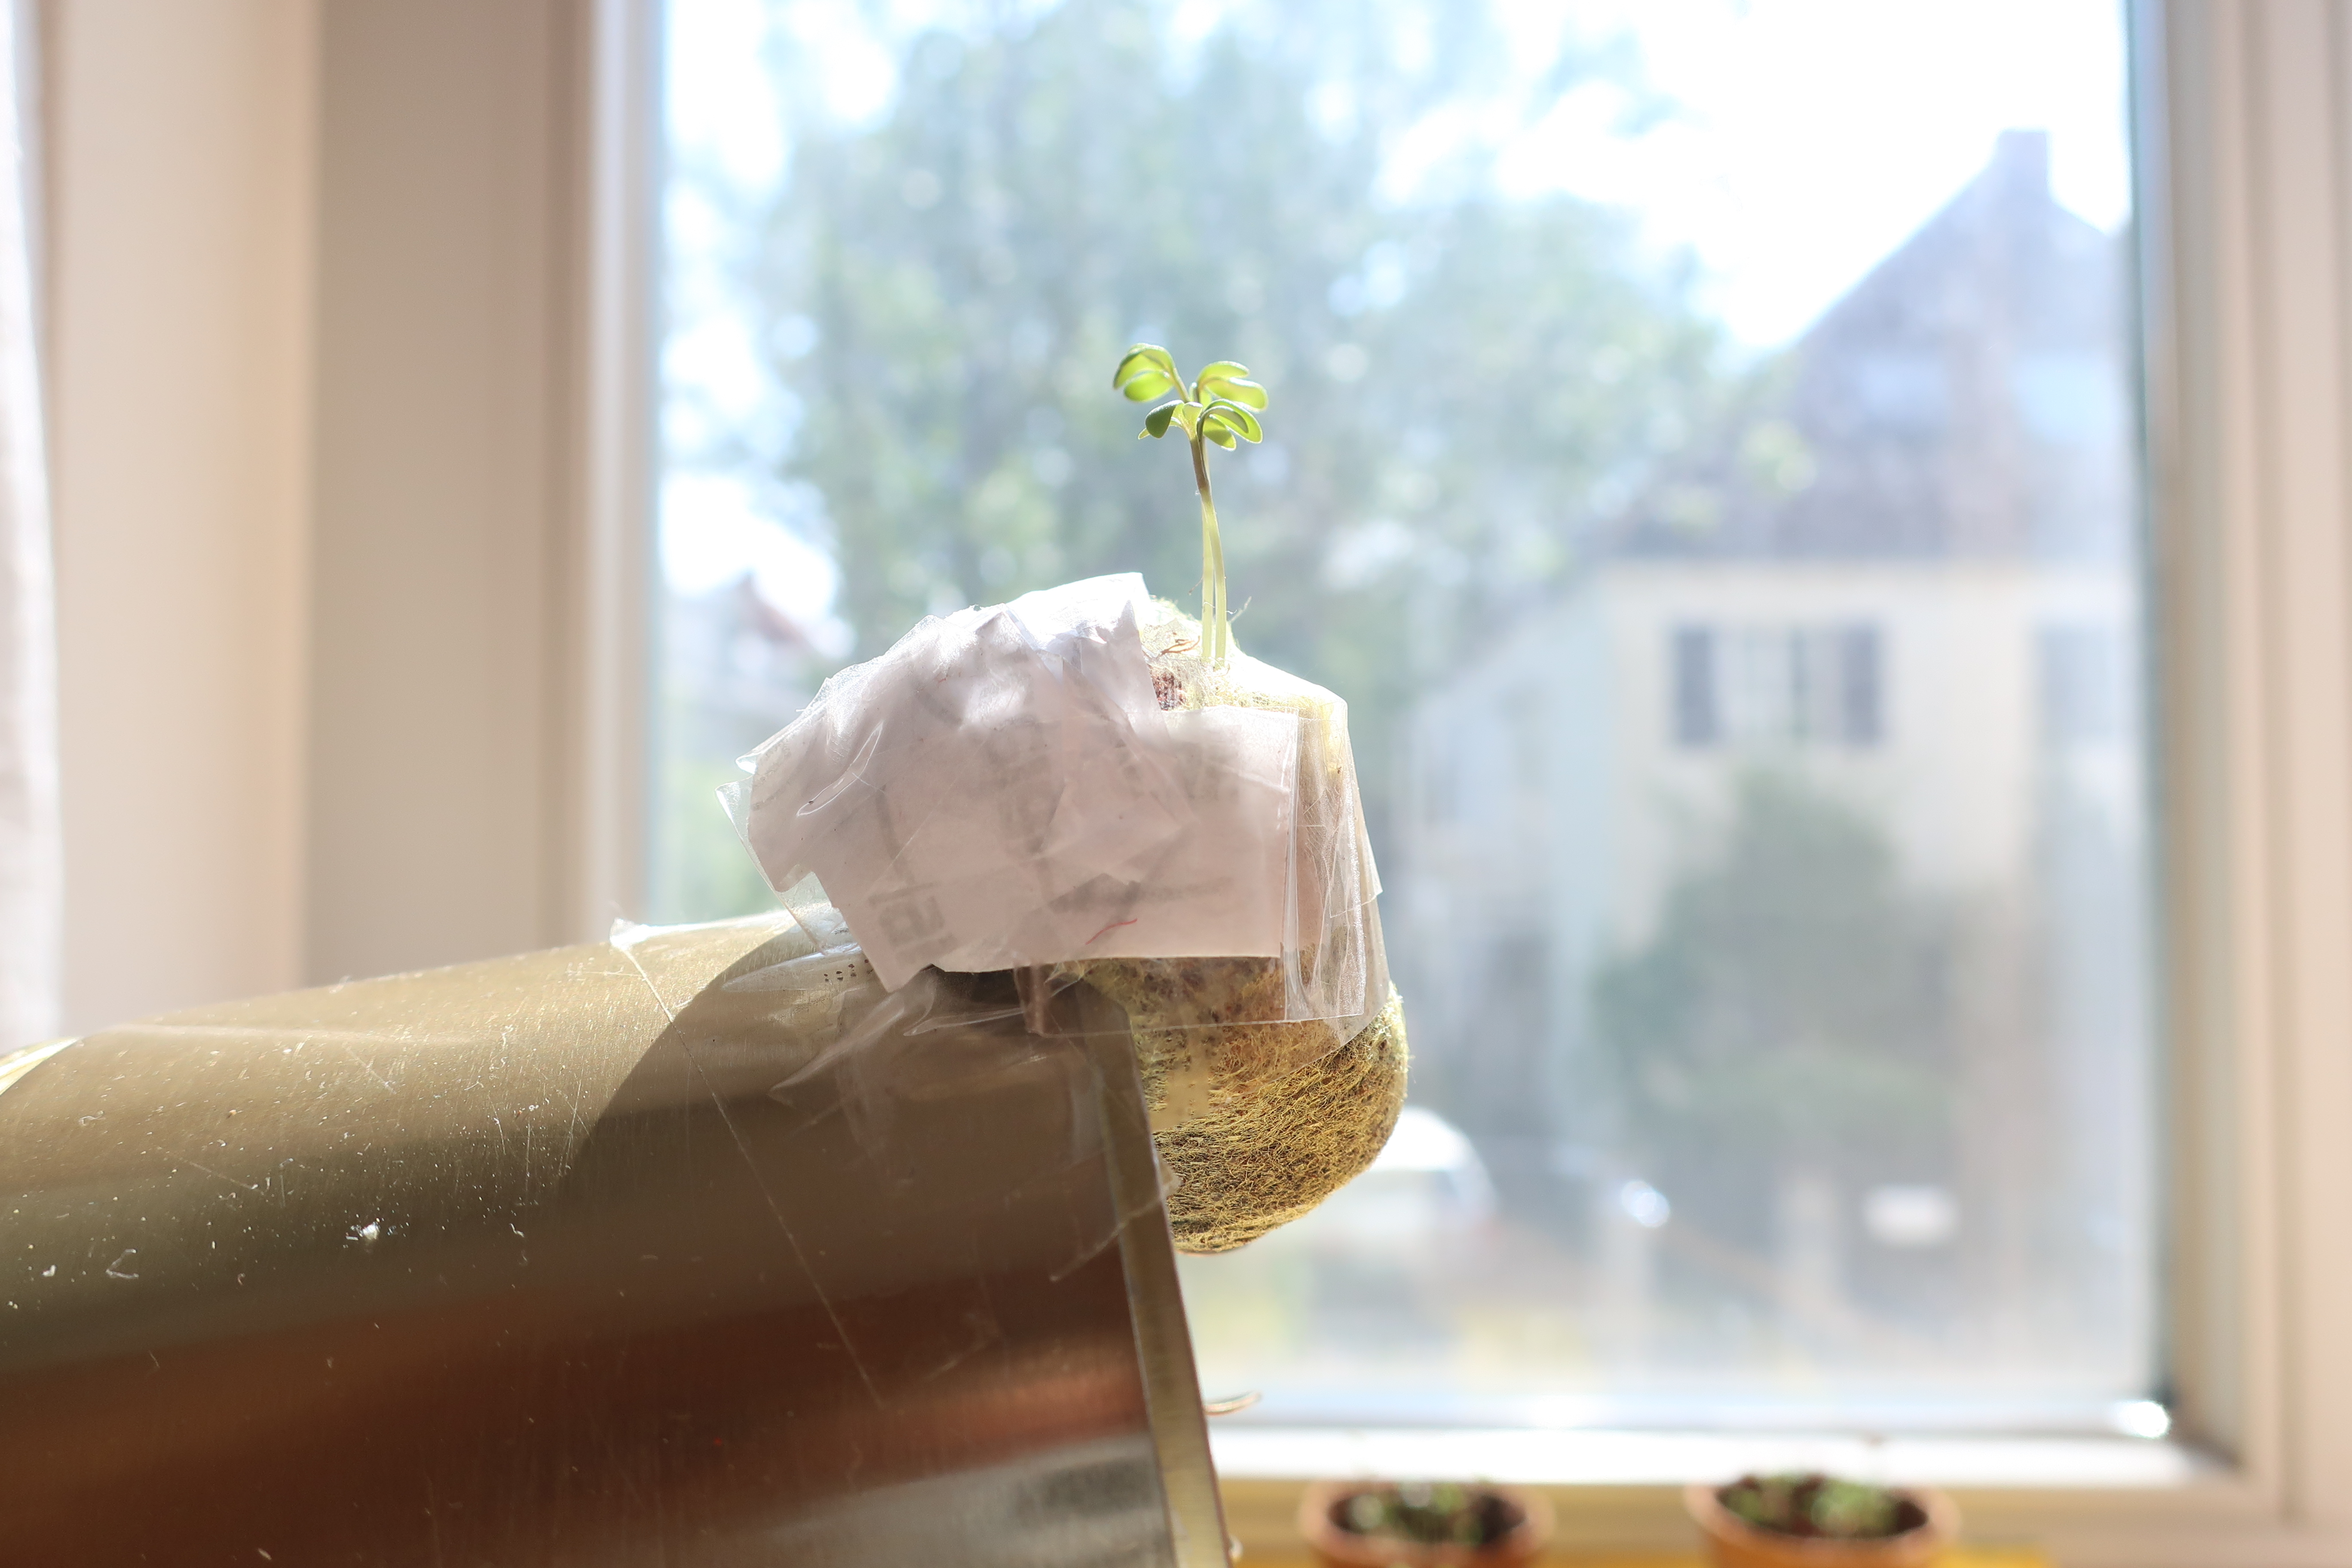
\includegraphics [width = .5\linewidth]{images/IMG_1083.JPG}
%  \end {figure} 
% Photo 1
%
% \begin{figure}
%  \centuring 
%  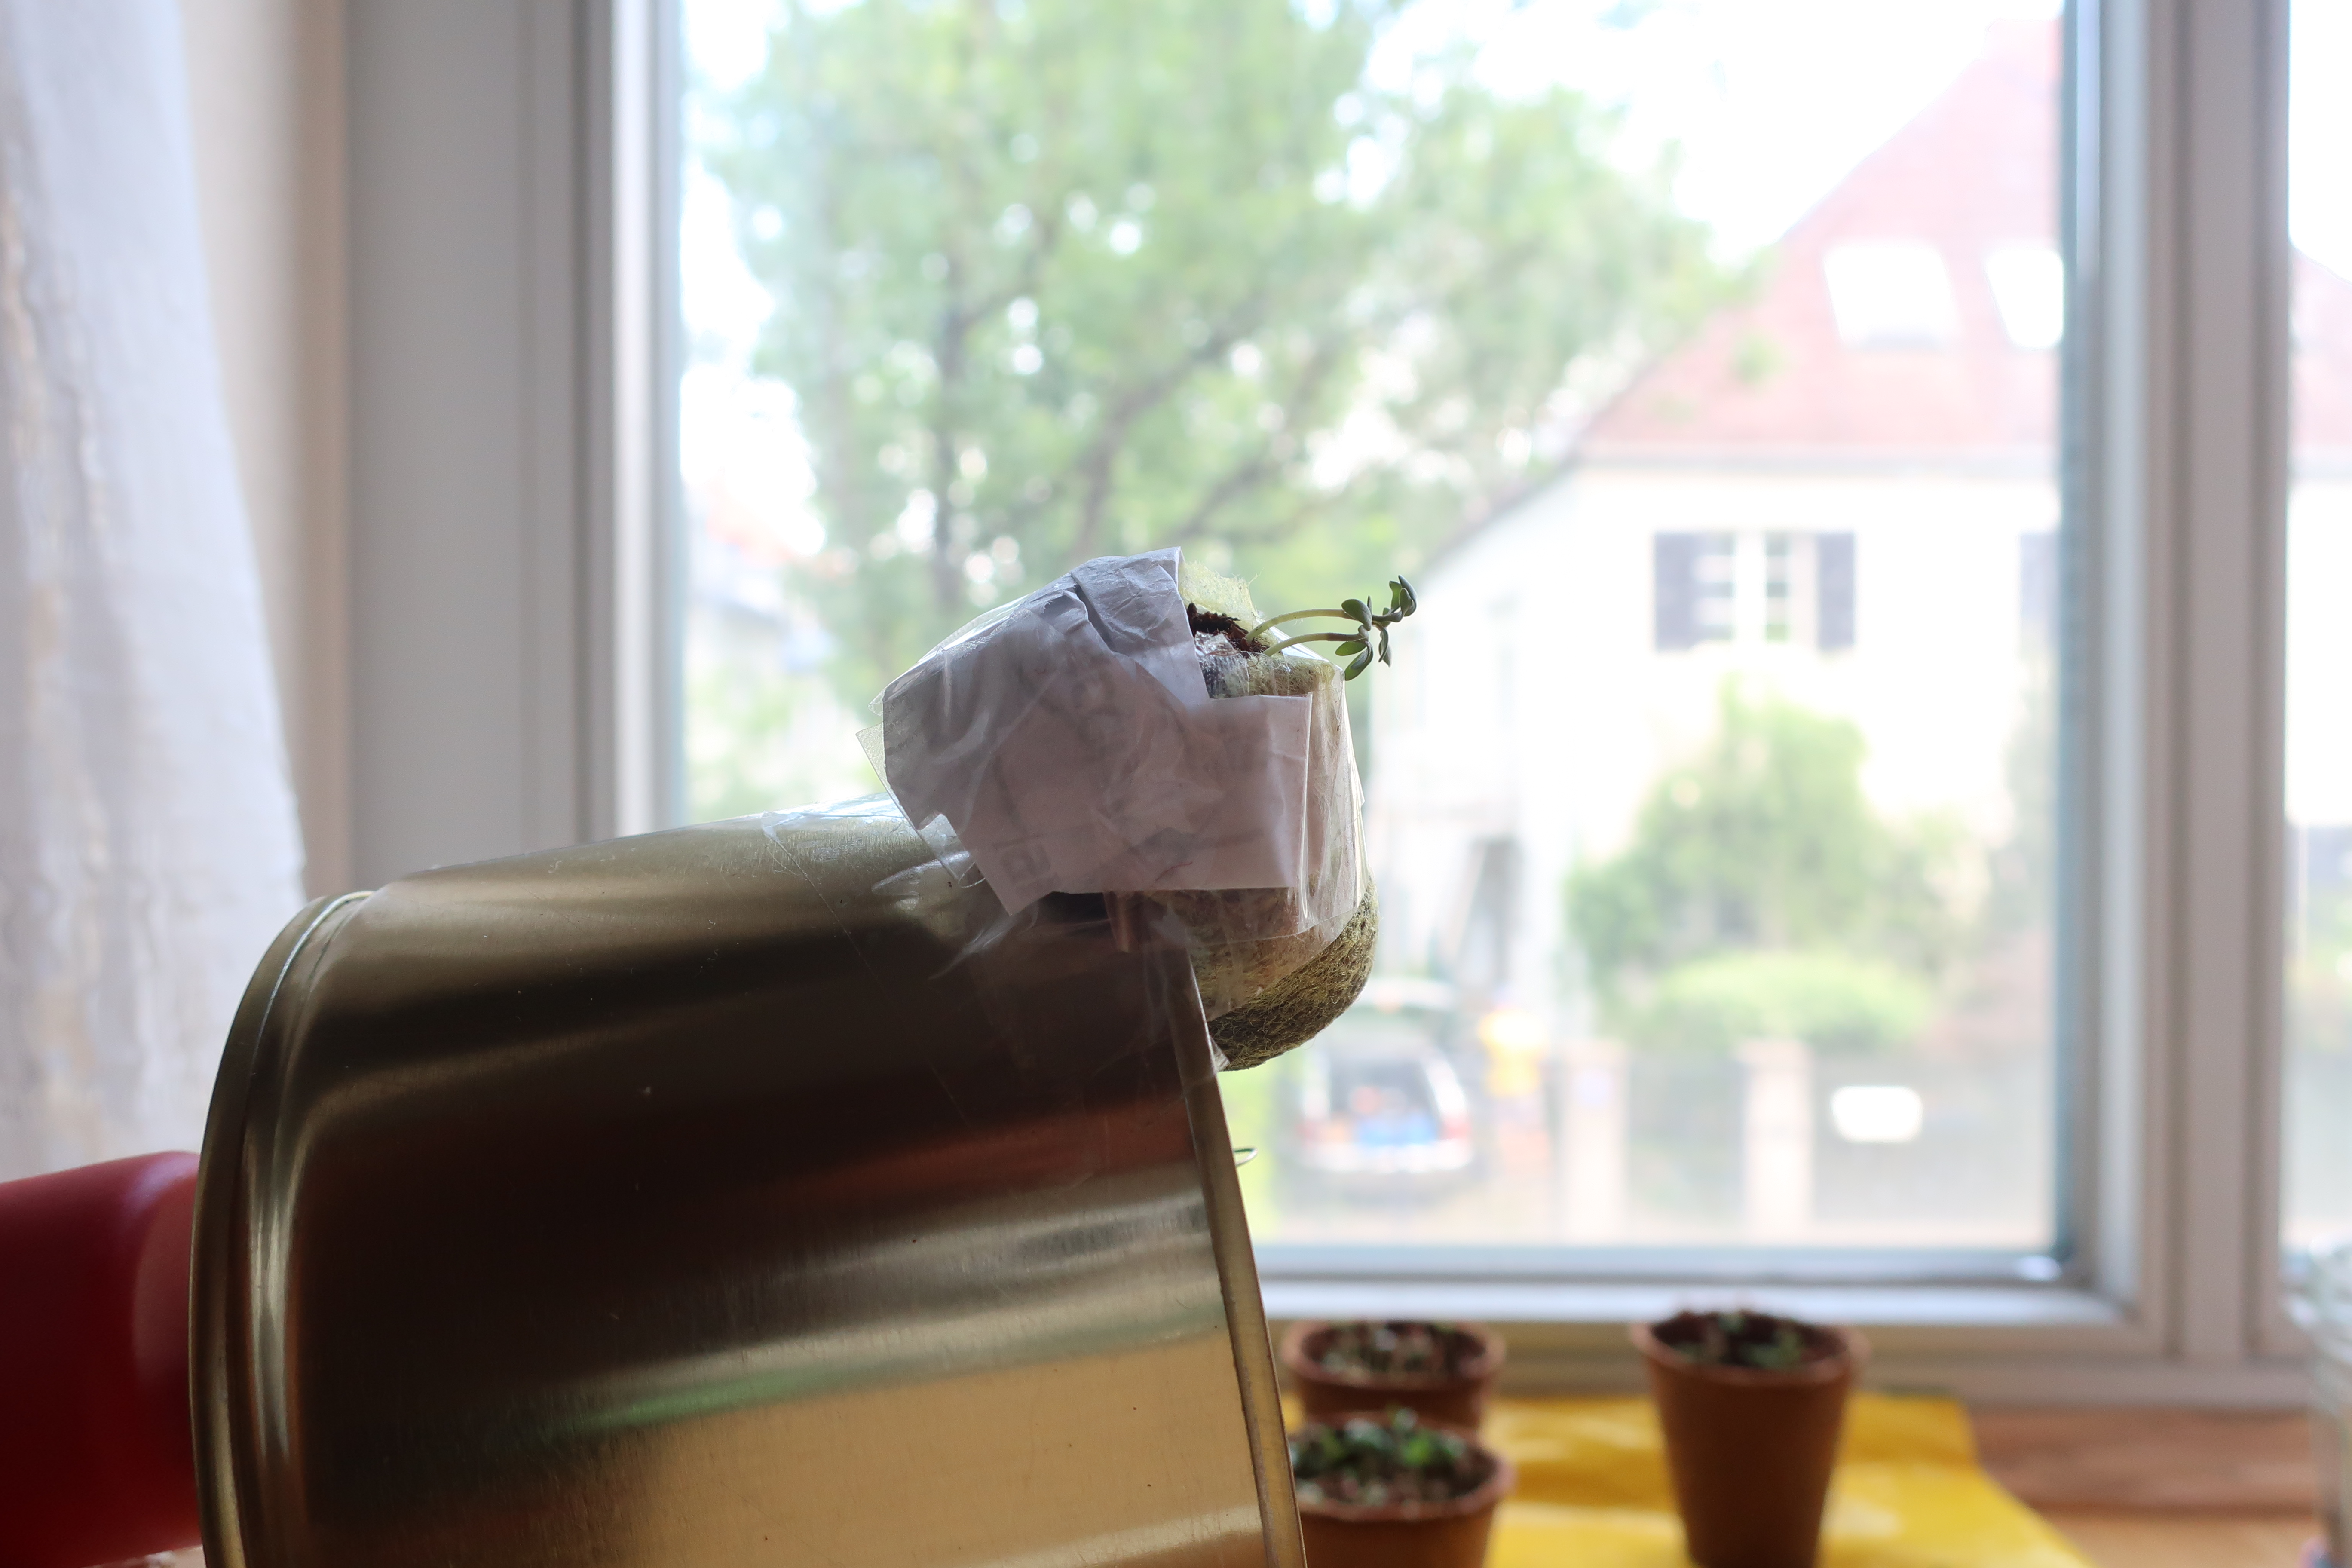
\includegraphics [width = .5\linewidth]{images/IMG_1073.JPG}
%  \end {figure} 
% Photo 2

%\begin{figure}
	%  \centuring 
	%  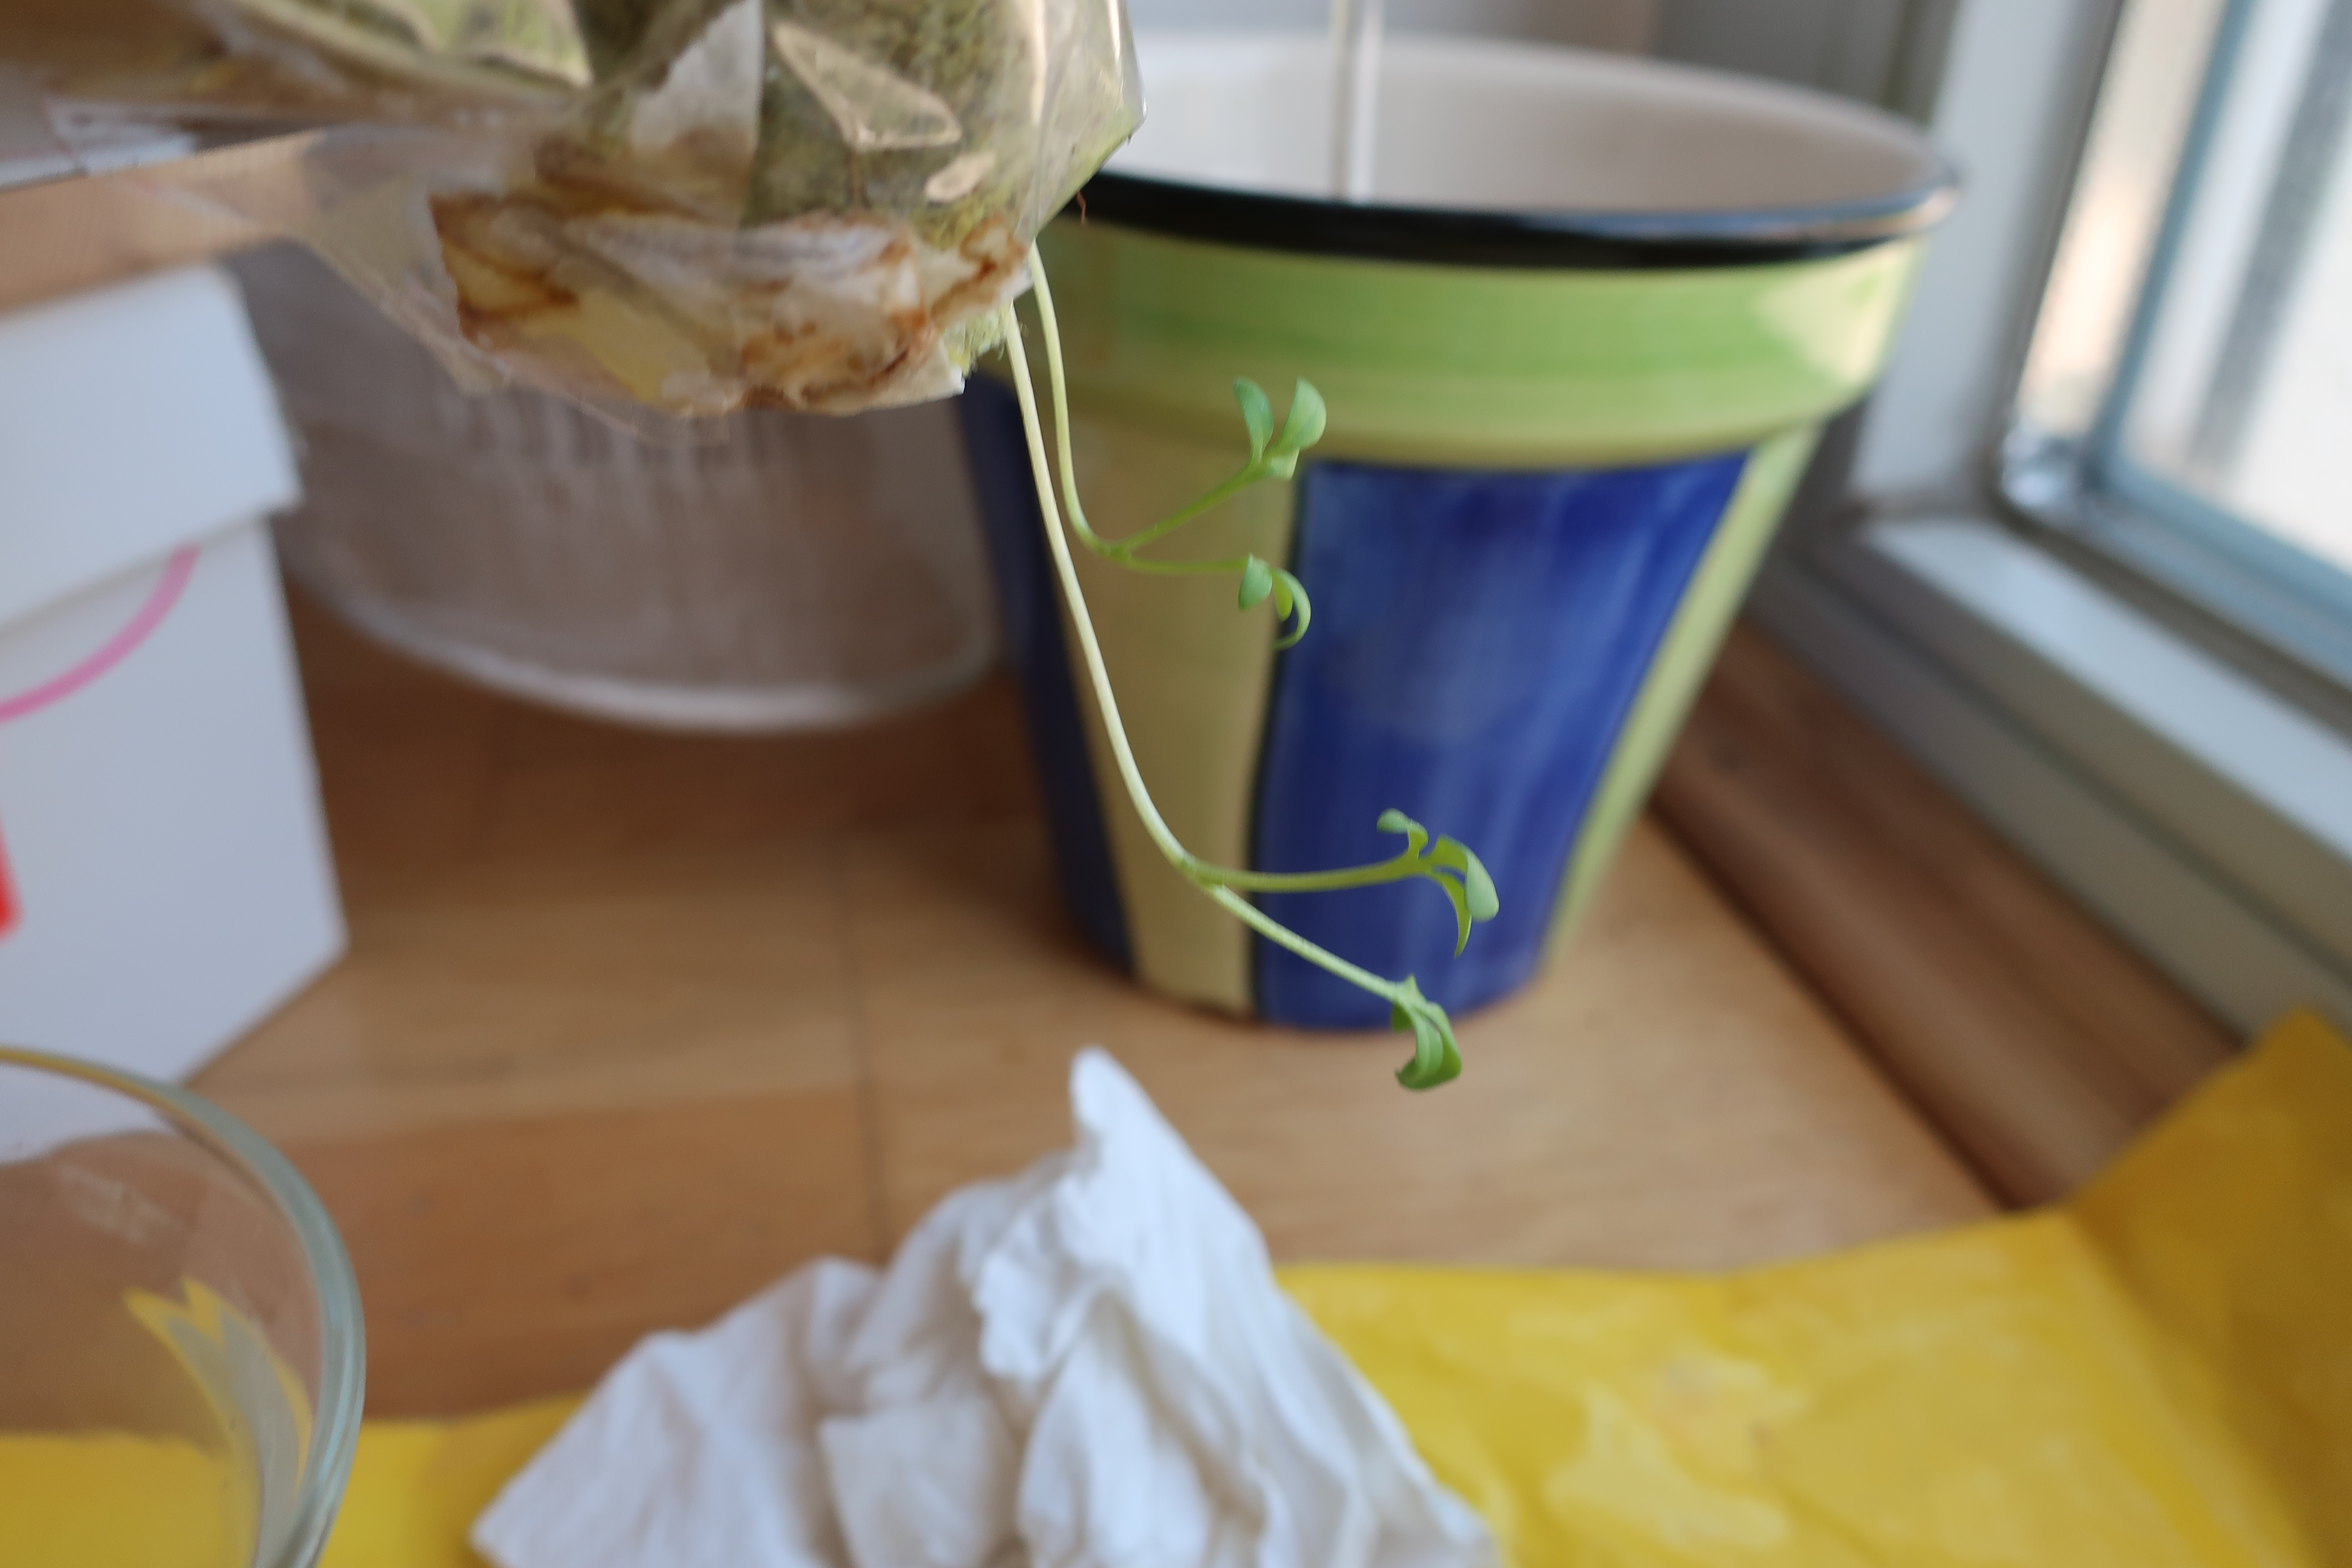
\includegraphics [width =.5\linewidth]{images/IMG_1399.JPG}
	%  \end {figure} 
	% Photo 5

\end{document}
